\RequirePackage[l2tabu, orthodox]{nag}
%\pdfminorversion=4
\documentclass[a0paper,portrait,fontscale=0.35]{baposter}

\usepackage{amsfonts,amsmath,amsthm,amssymb,commath}
\usepackage{graphicx,subcaption}
\usepackage[most,skins,theorems]{tcolorbox}
\usepackage{color}

\usepackage{relsize}
\usepackage{natbib}
\usepackage{microtype}

\usepackage{tikz}
\usetikzlibrary{decorations.pathreplacing}

%%% Define a caption font
\newcommand{\mycaption}[1]{
  {
    \smaller
    \emph{#1}
  }
}

\theoremstyle{plain}
\newtheorem{thm}{\protect\theoremname}
  \theoremstyle{plain}
  \newtheorem{lem}[thm]{\protect\lemmaname}
  \theoremstyle{definition}
  \newtheorem{defn}[thm]{\protect\definitionname}
  \theoremstyle{plain}
  \newtheorem{prop}[thm]{\protect\propositionname}
  \theoremstyle{definition}
  \newtheorem{example}[thm]{\protect\examplename}

%%% Color Definitions %%%%%%%%%%%%%%%%%%%%%%%%%%%%%%%%%%%%%%%%%%%%%%%%%%%%%%%%%
%\definecolor{oxford_blue}{RGB}{14,31,71}
%\definecolor{oxford_border}{RGB}{14,31,71}

%\definecolor{cambridge_blue}{RGB}{64,76,0}
%\definecolor{cambridge_blue}{RGB}{163, 193, 173}
%\definecolor{cambridge_border}{RGB}{163, 193, 173}

\definecolor{cambridge_blue}{RGB}{49,72,56}
\definecolor{cambridge_border}{RGB}{49,72,56}

\tcbset{highlight math style={enhanced, 
    colframe=cambridge_blue, colback=white}}

\begin{document}
\typeout{Poster rendering started}

\begin{poster}
{
    % Show grid to help with alignment
    grid=false,
    columns=6,
    % Column spacing
    colspacing=0.7em,
    % Color style
    %headerColorOne=cyan!20!white!90!black,
    %borderColor=cyan!30!white!90!black,
    headerColorOne=cambridge_blue,
    borderColor=cambridge_border,
    headerFontColor=white,
    % Format of textbox
    textborder=faded,
    % Format of text header
    headerborder=open,
    headershape=smallrounded,
    headershade=plain,
    background=none,
    bgColorOne=cyan!10!white,
    %headerheight=0.11\textheight,
    headerheight=0.095\textheight,
    eyecatcher=false,
}
% Eye Catcher: Oxford logo and personal picture
{
%  \makebox[0.23\textwidth]{
%    \begin{tabular}{cc}
%    \includegraphics[height=0.055\textheight]{./img/InFoMM}
%      &
%    %\includegraphics[height=0.10\textheight]{./img/me}
%    \end{tabular}
%    \hfill
%  }
}
%%% Title %%%%%%%%%%%%%%%%%%%%%%%%%%%%%%%%%%%%%%%%%%%%%%%%%%%%%%%%%%%%%%%%%%%%%
{
  %%\textsc{Source Reconstruction \vspace{0.2cm}\\From Hydrophone Data}
  \textsc{Spatially Variable Deconvolution\vspace{0.2cm}\\ 
    for Lightsheet Microscopy\vspace{0.2em}}
  \vspace{0.3em}
}
%%% Authors %%%%%%%%%%%%%%%%%%%%%%%%%%%%%%%%%%%%%%%%%%%%%%%%%%%%%%%%%%%%%%%%%%%
{
  \vspace{0.1em}
  \hspace{-0.65em}
  {
    \underline{\textbf{Bogdan Toader}}\textsuperscript{1},
    \textbf{St\'{e}phane Chr\'{e}tien}\textsuperscript{2}, 
    \textbf{Andrew Thompson}\textsuperscript{3}
  } \\[0.2em]
  {
    \textsuperscript{1}University of Cambridge,
    \textsuperscript{2}University of Lyon 2, 
    \textsuperscript{3}National Physical Laboratory
  }
}
%%% InFoMM Logo %%%%%%%%%%%%%%%%%%%%%%%%%%%%%%%%%%%%%%%%%%%%%%%%%%%%%%%%%%%%%%%
%{
%  %\makebox[0.23\textwidth]{
%  \makebox[0.32\textwidth]{
%    \hfill
%    \begin{tabular}{ccc}
%    %\includegraphics[height=0.055\textheight]{./img/InFoMM}
%      \includegraphics[height=0.04\textheight]{./img/InFoMM}
%      &
%    %\includegraphics[height=0.10\textheight]{./img/me}
%      \includegraphics[height=0.04\textheight]{./img/oxlogo}
%      \\
%      \includegraphics[height=0.04\textheight]{./img/turinglogo2}
%      &
%      \includegraphics[height=0.04\textheight]{./img/edinlogo}
%      %&
%      %\includegraphics[height=0.05\textheight]{./img/me_square}
%    \end{tabular}
%  }
%  %}
%}
{
  %\makebox[0.23\textwidth]{
  \makebox[0.32\textwidth]{
    \hfill
    \begin{tabular}{ccc}
      \includegraphics[height=0.04\textheight]{./img/camlogo}
    \end{tabular}
  }
  %}
}
\headerbox{lightsheet microscopy}{name=lightsheet, span=3, column=0, row=0}{

  \begin{minipage}[t]{\textwidth}
    TODO: a few words about why lightsheet is good

    Light sheet microscopy is a type of fluorescence microscopy used in cell biology due to its fast acquisition times and low photo-damage to the sample. This is achieved by selectively illuminating a slice of the sample using a sheet of light and detecting the emitted fluorescence signal using a dedicated objective orthogonal to the plane of the sheet. 

    %Consequently, the effective point spread function (PSF) of the microscope is space varying, which adds an additional layer of complexity to the problem of deconvolution of such images.
     \begin{itemize} 
      \item
        Project aim: computationally improve the 
        quality of light sheet microscopy images.
    \end{itemize}

  \end{minipage}
  \vspace{1pt}
    
  \begin{minipage}[t]{\textwidth}
    \begin{minipage}[t]{0.48\textwidth}
      \begin{center}
        \larger
        {\color{blue}\textbf{\textsc{Light-sheet microscope}}}\\
        %\textit{$x$ is the discrete measure\\
        %we want to reconstruct.}
      \end{center}
          
      \begin{minipage}[t]{\textwidth}
        \centering
        \includegraphics[width=\textwidth]{img/spim.png}
       
        \mycaption{Figure credit: J\"{o}rg Ritter, PhD thesis (2011)}
        %\mycaption{The input signal is a sum of Diracs \\ represented 
         % as a discrete measure.}
      \end{minipage}
     
      %\vspace{-0.5em}
      %\begin{center}
      %  \tcbhighmath[colback=blue!10!white, frame hidden]{
      %    x(t) = \sum_{i=1}^{k} a_i \cdot \delta_{t_i},
      %    %\quad a_i > 0
      %  }
      %\end{center}

      \hspace{1em}
      %{ \smaller 
      %  $t_i$ and $a_i$ ($i=1,\ldots,k$) are the locations\\
      %  and magnitudes of the point sources.}
      
      A light-sheet microscope consists of two objectives: TODO etc
    
    \end{minipage}
    %
    \begin{minipage}[t]{0.48\textwidth}
      \begin{center}
        \larger
        {\color{blue}\textbf{\textsc{Spatially varying PSF}}}\\
        %\textit{$y_i$ are the samples\\
        %  we use to reconstruct $x$.}
      \end{center}
      
      \begin{minipage}[t]{\textwidth}
        \centering
        \includegraphics[width=\textwidth]{img/psf_4.png}

        %\mycaption{The measured signal is the convolution of the \\ input signal
        %  with a window function $\psi$.}
      \end{minipage}

      \begin{center}
        \larger
        {\color{red}\textbf{\textsc{Problem}}}\\
      \end{center}
      \vspace{-0.5em}
      \begin{tcolorbox}[colback=red!10!white,colframe=red]
        Due to the combination of light-sheet and the objective PSF, 
        the effective PSF of the system is spatially varying, and
        therefore standard deconvolution approaches are not applicable.
      \end{tcolorbox}

    \end{minipage}
  \end{minipage}
}
\headerbox{model}{name=model, span=3, column=3, row=0}{

  \begin{minipage}[t]{\textwidth}
    The measure $x$ can be recovered exactly by solving 
    the TV norm minimisation problem over non-negative
    measures $z$ on $[0,1]$:
    \begin{tcolorbox}[colback=teal!10!white,colframe=white]
      \begin{equation}
        \min_{z \geq 0} \|z\|_{TV} 
        \quad \text{subject to} \quad
        y_j = \int_{[0,1]} \phi(t-s_j)x(\dif t),
        \quad
        \forall j=1,\ldots,m,
      \end{equation}
    \end{tcolorbox}
    or its dual:
    \begin{tcolorbox}[colback=teal!10!white,colframe=white]
      \begin{equation}
        \max_{\lambda \in \mathbb{R}^m}
        y^T \lambda 
        \quad \text{subject to} \quad
        \sum_{j=1}^m \lambda_j \phi(t-s_j) \leq 1,
        \quad \forall t \in [0,1].
        \label{eq:dual}
      \end{equation}
    \end{tcolorbox}
  \end{minipage}
  %\vspace{-10pt}
  \begin{minipage}[t]{\textwidth}
    \begin{minipage}[h]{0.53\textwidth} 
      Having the solution $\lambda$ to the dual problem \eqref{eq:dual},
      the locations $\{t_i\}_{i=1}^k$ in the input signal
      are given by the global maximisers of the dual certificate:
      \vspace{-0.5em}
      \begin{center}
        \tcbhighmath[colback=red!10!white, frame hidden]{
          q(t) = \sum_{j=1}^m \lambda_j \phi(t-s_j).
        }
      \end{center}
    \end{minipage}
    %
    \begin{minipage}[h]{0.44\textwidth}
      \centering
      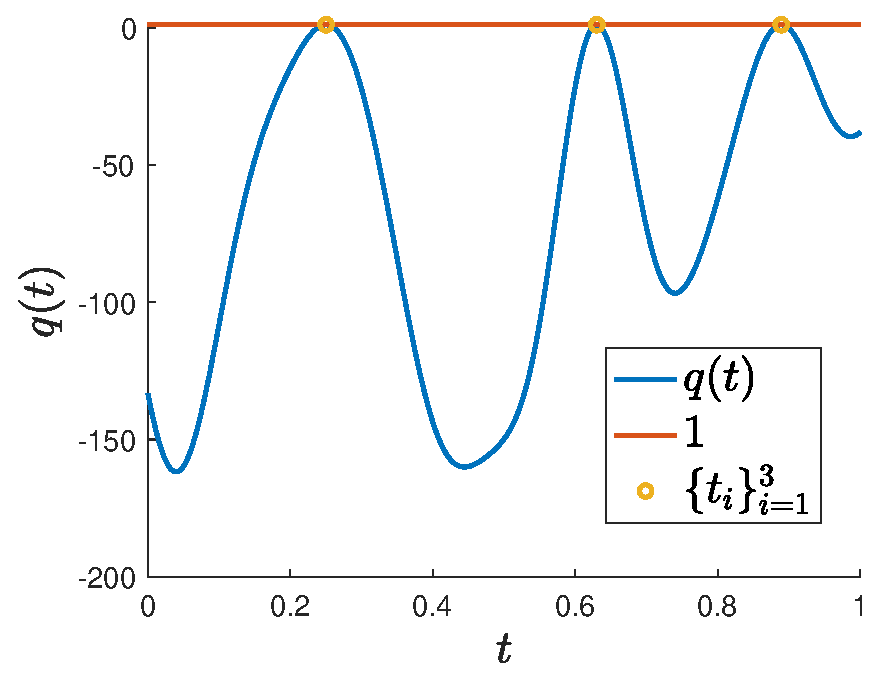
\includegraphics[height=0.097\textheight]{img/dual_certif.eps}
    \end{minipage}
  \end{minipage} 
}

\headerbox{Fitting the PSF}{name=psf, span=3, column=0, below=lightsheet}{
  \begin{minipage}[t]{\textwidth} 
    \begin{center}
      \larger
      \textbf{\textsc{Algorithm}}
    \end{center}

    We solve 
    %\begin{center}
      \tcbhighmath[colback=teal!10!white, frame hidden]{
        \min_{\lambda \in \mathbb{R}^m} f(\lambda)
      }
    %\end{center}
    %where $f(\lambda)$ is the exact penalty formulation
    %of the dual:
    for the exact penalty $f$:
    \begin{center}
      \tcbhighmath[colback=red!10!white, frame hidden]{
        f(\lambda) = 
        -y^T \lambda
        + \Pi \cdot
        \max\{
          \sup_{s} \sum_{j=1}^m
            \lambda_j \phi(s-s_j) - 1,
          0
        \}
      }
    \end{center}
    in the set 
    $ Q = \{ \lambda \in \mathbb{R}^m ~|~ 
        \|\lambda\|_{\infty} \leq B \} $.
    %\begin{minipage}[t]{\textwidth}
    As described in \cite{NesterovOpt}, at every iteration $p$:
      \begin{enumerate}
        \item Compute the piece-wise linear model:  
          \begin{equation*}
            \hat{f}_p(\lambda) = \max_{0\leq l \leq p} \left[
              f(\lambda_l) + \left< g(\lambda_l), \lambda-\lambda_l \right>
            \right],
          \end{equation*}
          where $g(\lambda_l)$ are some subgradients of $f$ at $\lambda_l$.

       \item Find the optimal value $\hat{f}_p^*$ of the current 
         model $\hat{f}_p$ and
          the smallest value $f_p^*$ of the objective $f$ so far.
          %Note that $\hat{f}_p^* \leq f_p^*$.

        \item Calculate the next iterate $\lambda_{p+1}$ as the projection
          of $\lambda_p$ on the level set 
          $
            \mathcal{L}_p(\alpha) = \{\lambda \in Q ~|~ 
              \hat{f}_p(\lambda) \leq \ell_p(\alpha)\}
          $
          where 
          $
            \ell_p(\alpha) = (1-\alpha)\hat{f}_p^* + \alpha f_p^*
          $
          for some $\alpha \in (0,1)$.
      \end{enumerate}
    %\end{minipage}
  \end{minipage}
  %
%  \hspace{0.7em}
%  \begin{minipage}[t]{0.66\textwidth}
%    \begin{minipage}[t]{0.33\textwidth}
%      \begin{center}
%        \larger
%        \textbf{\textsc{Theorem 1}}
%      \end{center}
%      \vspace{-0.7em}
%     
%      \begin{tcolorbox}[colback=teal!10!white,colframe=cambridge_blue]
%        Perturbations $\tilde{t_i}$ of the source 
%        locations $t_i^*$ are bounded explicitly as a function 
%        of the perturbations in the dual variable $\lambda$ around the 
%        solution $\lambda^*$:
%
%        \begin{equation*}
%          \frac{|\tilde{t}_i-t^*_i|}{\|\tilde{\lambda}-\lambda^*\|_2} 
%          \leq C_{t^*}
%        \end{equation*}
%      \end{tcolorbox}
%   
%      \begin{minipage}[t]{\textwidth}
%        \centering
%
%        \includegraphics[height=0.10\textheight]{img/t_lam.eps}
%        %\vspace{-1.5em}
%        %\mycaption{(a)}
%      \end{minipage}
%
%    \end{minipage}
%    \begin{minipage}[t]{0.33\textwidth}
%      \begin{center}
%        \larger
%        \textbf{\textsc{Theorem 2}}
%      \end{center}
%      \vspace{-0.7em}
%     
%      \begin{tcolorbox}[colback=teal!10!white,colframe=cambridge_blue]
%        Perturbations $\mathbf{\tilde{a}}$ of the source 
%        weights $\mathbf{a^*}$ are bounded explicitly as a function
%        of the perturbations $\mathbf{\tilde{t}}$ in the 
%        true source locations $\mathbf{t^*}$:
%       
%        \vspace{0.5em}
%        \begin{equation*} 
%          \frac{\|\mathbf{\tilde{a}}-\mathbf{a^*}\|_2}{
%            \|\mathbf{\tilde{t}}-\mathbf{t^*}\|_2
%          } 
%          \leq C_{a^*} 
%          + \mathcal{O}(\|\mathbf{\tilde{t}}-\mathbf{t^*}\|_2)
%        \end{equation*}
%      \end{tcolorbox}
%
%      \begin{minipage}[t]{\textwidth}
%        \centering
%
%        \includegraphics[height=0.10\textheight]{img/a_t.eps}
%        %\vspace{-1.5em}
%        %\mycaption{(b)}
%      \end{minipage}
%    
%    \end{minipage}
%    \begin{minipage}[t]{0.33\textwidth}
%      \begin{center}
%        \larger
%        \textbf{\textsc{Theorem 3}}
%      \end{center}
%      \vspace{-0.7em}
%     
%      \begin{tcolorbox}[colback=teal!10!white,colframe=cambridge_blue]
%        Perturbations of the dual variable $\lambda$ around 
%        the solution $\lambda^*$ of the dual problem are
%        bounded explicitly as a function of the 
%        additive noise $\mathbf{w}$ in the measurements:
%        
%        \vspace{0.2em}
%        \begin{equation*}
%          \frac{\|\tilde{\lambda}-\lambda^*\|_2}{
%            \|\mathbf{w}\|_2
%          }
%          \leq C_{\lambda^*}
%        \end{equation*}
%      \end{tcolorbox}
%    
%      \begin{minipage}[t]{\textwidth}
%        \centering
%
%        \includegraphics[height=0.10\textheight]{img/lam_w}
%        %\vspace{-1.5em}
%        %\mycaption{(c)}
%      \end{minipage}
%    \end{minipage}
%    \vspace{-0.9em}
%    \begin{center} 
%      \mycaption{ 
%        The error ratios from the theorems above 
%        when applying the level method to the dual problem
%        for source\\ 
%        locations $t_i \in \{0.25, 0.63, 0.888\}$,
%        weights $a_i \in \{0.8,0.5,0.9\}$,
%        $m=21$ equispaced samples in $[0,1]$ and\\
%        Gaussian kernel $\phi(t) = e^{-t^2/\sigma^2}$
%        with $\sigma = 0.07$.
%        Left: $t_2$,$\lambda$,
%        middle: $a$,$t$,
%        right: $\lambda$,$w$.\\
%        The exact conditions in which the results above hold, 
%        together with the explicit expressions for the\\
%        constants $C_{t^*}$, $C_{a^*}$ and $C_{\lambda^*}$
%        respectively are given in \cite{chretien2019dual}.
%      }
%    \end{center}
%  \end{minipage}
}

\headerbox{Results -- simulated data}{name=resultssim, span=3, column=3, below=model}{



}

\headerbox{Results -- real data}
{name=resultsreal,column=0, below=psf, span=6}{
  \begin{minipage}[t]{0.51\textwidth} 
    \begin{center}
      \larger
      \textbf{\textsc{Beads}}
    \end{center}

    \vspace{-1em}
    \begin{minipage}[h]{0.5\textwidth}
      \begin{itemize}
        \item \textbf{Exact measurements:} 
          the level method finds the correct
          locations of the point sources with high
          accuracy -- see the localisation error
          for two sources as the distance between them
          goes to zero in the bottom left figure. 
        \item \textbf{Noisy measurements:}
          As the distance between two sources
          decreases, they are replaced with one source
          with higher intensity in the reconstructed
          signal.
      \end{itemize}
    \end{minipage}
    %
    \begin{minipage}[h]{0.49\textwidth}
      \centering
      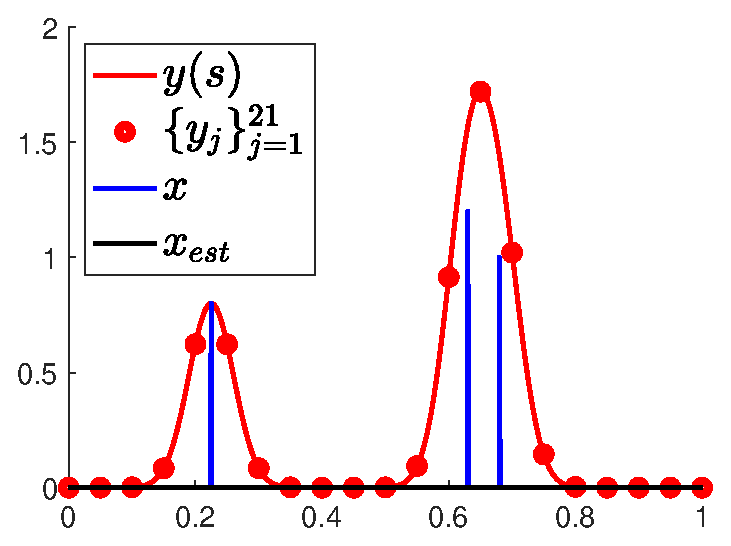
\includegraphics[height=0.1\textheight]{img/1d_base.eps}
      %\vspace{-0.5em}
      
      \mycaption{Example of setup with noise-free\\ 
        measurements, solved to accuracy $10^{-6}$.}
    \end{minipage}
 
    \vspace{0.5em}
    \begin{minipage}[h]{0.97\textwidth}
      \begin{minipage}[h]{0.5\textwidth}
        \centering
        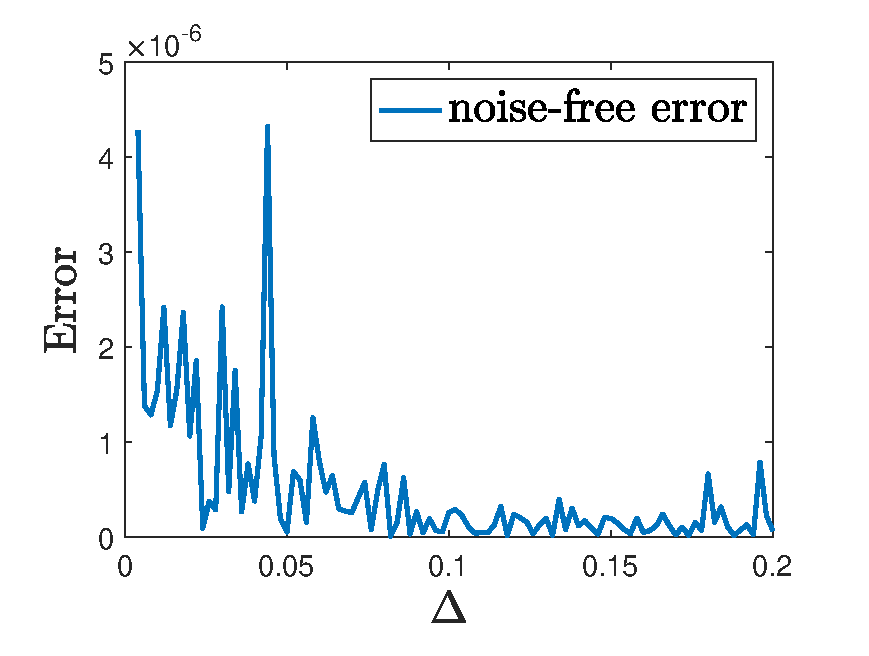
\includegraphics[height=0.12\textheight]{img/1d_error_noisefree.eps}
        %\vspace{-0.5em}
      \end{minipage}
      %
      \begin{minipage}[h]{0.5\textwidth}
        \centering
        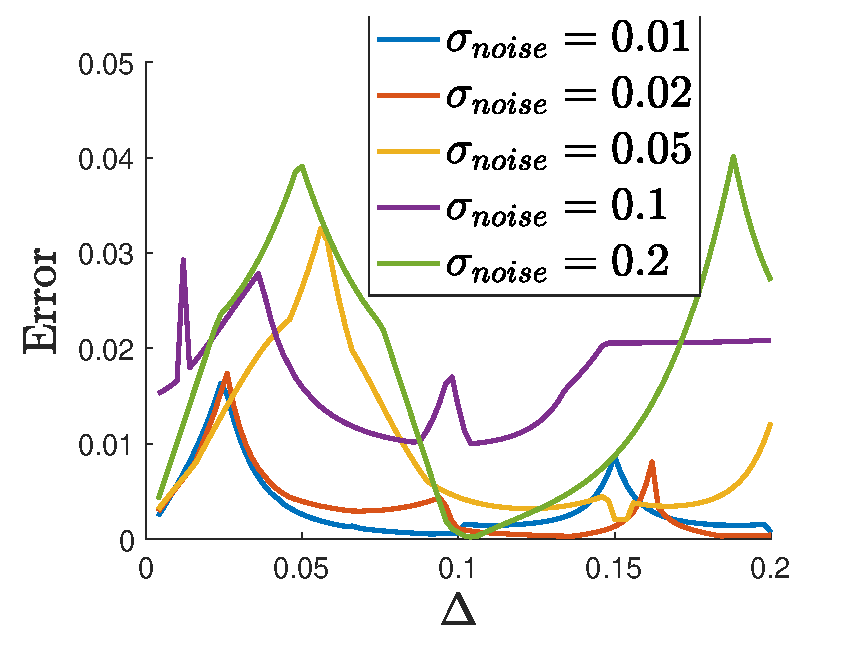
\includegraphics[height=0.12\textheight]{img/1d_error_noisy.eps}
        %\vspace{-0.5em}
      \end{minipage}

      \vspace{-1em}
      \begin{center}
        \mycaption{Localisation error for two point sources
          as the distance $\Delta$ between them increases 
          from $0.004$ to $0.2$ in the noise-free case (left)
          and noisy case for Gaussian noise with standard deviation
          $0.01$, $0.02$, $0.05$, $0.1$, $0.2$ (right).
          The convolution kernel
          is Gaussian with $\sigma=0.05$, intensities are $1$ 
          and $m=21$ equispaced samples.
        }
        \end{center}
    \end{minipage}
  \end{minipage}
  %
  \begin{minipage}[t]{0.48\textwidth}
    \begin{center}
      \larger
      \textbf{\textsc{Marchantia}}
    \end{center}
    
    \begin{minipage}[h]{\textwidth}
      Examples of $k=25$ sources in an image with $67 \times 67$ 
      pixels (giving $m=4489$ measurements), Gaussian kernel
      with $\sigma = 0.05$ and level method parameters
      $\Pi = 100$ and $B = 100$.
      Red crosses 
        \includegraphics[height=0.007\textheight]{img/cross.png}
       are true sources and 
      black circles 
        \includegraphics[height=0.007\textheight]{img/circle.png}
       are estimated sources.
      
     \vspace{0.7em}
      \begin{minipage}[t]{0.49\textwidth}
        \centering
        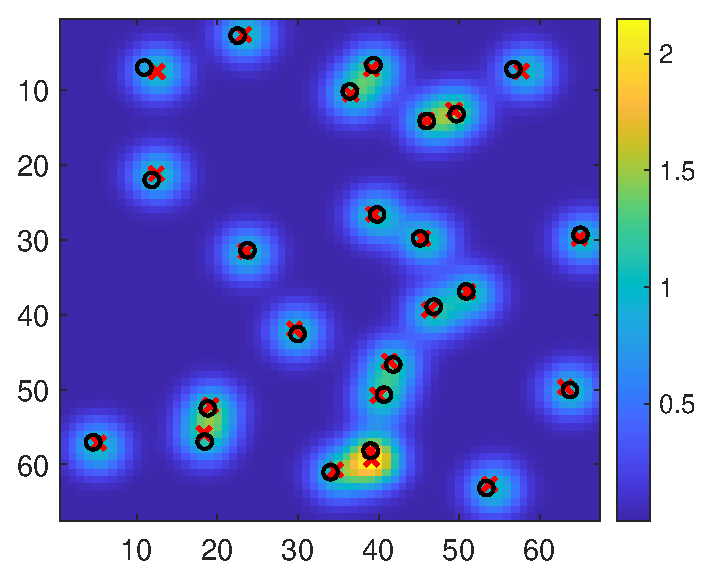
\includegraphics[height=0.1\textheight]{img/2d_noise_free_nolegend.eps}

        \vspace{-0.3em}
        \mycaption{
          Noise-free measurements.
        }
      \end{minipage}
      %
      \begin{minipage}[t]{0.49\textwidth}
        \centering
        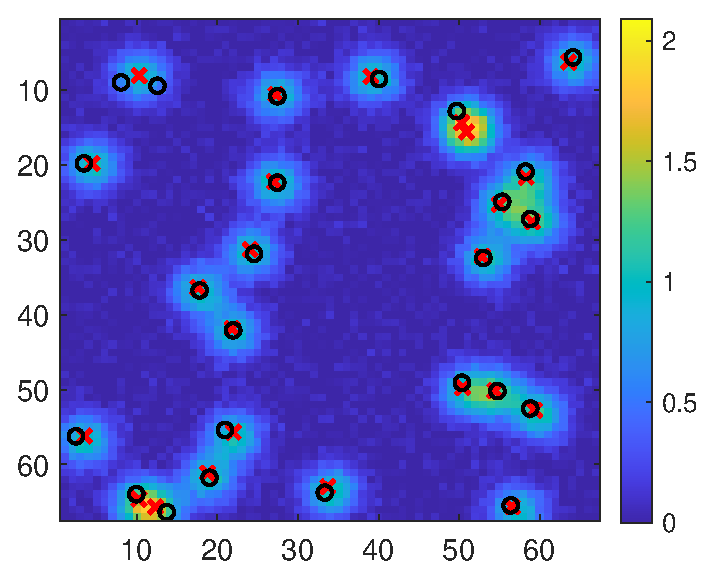
\includegraphics[height=0.1\textheight]{img/2d_noise_005_nolegend.eps}

        \vspace{-0.3em}
        \mycaption{
          Gaussian noise with standard deviation $0.05$.
        }
      \end{minipage}

      \vspace{0.9em}
      \begin{minipage}[t]{0.49\textwidth}
        \centering
        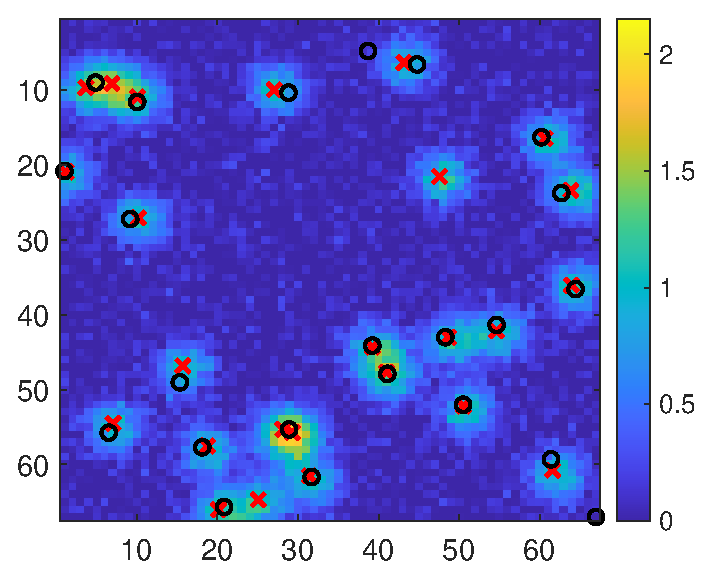
\includegraphics[height=0.1\textheight]{img/2d_noise_01_nolegend.eps}

        \vspace{-0.3em}
        \mycaption{
          Gaussian noise with standard deviation $0.1$.
        }
      \end{minipage}
      %
      \begin{minipage}[t]{0.49\textwidth}
        \centering
        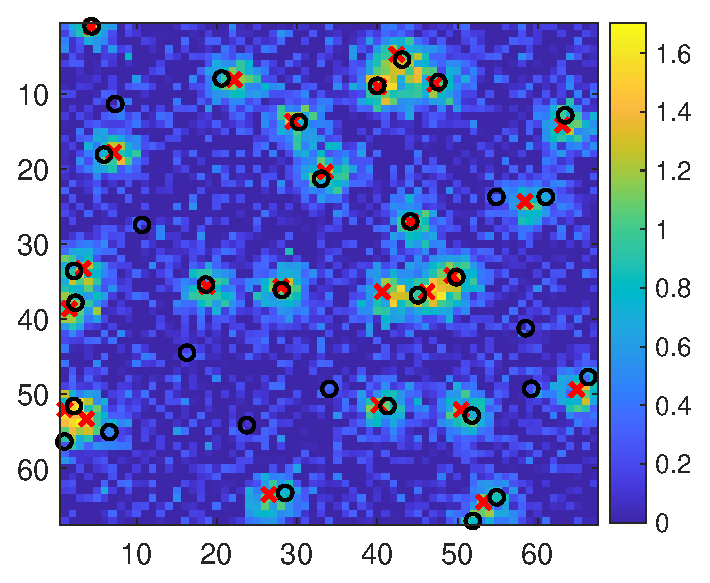
\includegraphics[height=0.1\textheight]{img/2d_noise_02_nolegend.eps}

        \vspace{-0.3em}
        \mycaption{
          Gaussian noise with standard deviation $0.2$.
        }
      \end{minipage}
    \end{minipage}
  \end{minipage}
  \vspace{-1em}
}

\headerbox{References}
{name=references, column=0,  below=resultsreal, span=3}
%{name=references, column=0,  above=bottom, span=1}
{
  %\smaller                                  % Make the whole text smaller
  %\footnotesize
  %\scriptsize
  \tiny
  \bibliographystyle{abbrv}                 % Use plain style
  \renewcommand{\section}[2]{\vspace{0.05em}}	% Omit "References" title
  \bibliography{references}
}

\headerbox{Acknowledgments}
{name=acknowledgments, column=3, below=resultsreal, span=3}
%{name=acknowledgments, column=1, above=bottom, span=1}
{  
  \scriptsize
  %\tiny
  This poster is based on work supported by 
  the EPSRC Centre For Doctoral Training in Industrially Focused Mathematical 
  Modelling (EP/L015803/1) in collaboration with the National Physical Laboratory 
  and by the Alan Turing Institute under the EPSRC grant EP/N510129/1.
  B.T is currently funded by  
  Isaac Newton Trust/Wellcome Trust ISSF/University of Cambridge 
  Joint Research Grants Scheme, RG89305.
%  \vspace{-0.6em}
%  \begin{center}
%    \begin{tabular}{cccc}
%      \includegraphics[height=0.02\textheight]{./img/epsrc_logo.eps}
%      &
%      \includegraphics[height=0.018\textheight]{./img/InFoMM}
%      &
%      \includegraphics[height=0.02\textheight]{./img/company_logo.jpg}
%      &
%      \includegraphics[height=0.018\textheight]{./img/turinglogo2.jpg}
%    \end{tabular}
%  \end{center}
  \par
}






\end{poster}
\end{document}

%%% Local Variables:
%%% mode: latex
%%% TeX-master: t
%%% End:
